\section{Pixelized Readout}
\label{chap:TPC_sec:pixels}
Most recent update: 2018-11-01 \\
Contact person: Klaus Desch (email: desch@physik.uni-bonn.de)\\

\subsection{Introduction}
To make the most of the fine pitches of the Micropattern Gaseous Detectors the
readout structure should be adapted to the same feature size. Therefore,
readout ASICs of silicon pixel detectors such as the Timepix ASIC
\cite{Llopart2007485, Llopart2008106} can be placed directly below the gas amplification
stage. In this setup, the bump bond pads normally used to connect the readout
chip to the Si-sensor are used as charge collection pads. In some studies a
triple GEM was used as a gas amplification stage \cite{Bamberger:2006xp, 6359808},
while in others a Micromegas has been built
directly on the ASIC \cite{4526754}. The latter detector type is 
 called GridPix and is produced by using a post-processing technique, which
 guarantees a high quality grid perfectly aligned with the readout pixels. This
 alignment ensures that the complete charge avalanche initiated by a primary
 electron is collected on one pixel. Because of the high signal-to-noise
 ratio both tracking and dE/dx measurement benefit from distinguishing and
 detecting single primary electrons with a high efficiency. This type of
 detector was pioneered by Nikhef/University of Twente (NL). The University
 of Bonn has modified the 
 production process together with the Fraunhofer Institut IZM so that a
 wafer-based production of GridPix detectors is standard by now
 \cite{Koppert2013245}. First tests were done with both
 gas amplification stages by using single ASICs with an active area of about \SI{2}{\centi\meter\squared}. The detectors were operated in laboratories at Nikhef, Saclay, Bonn,
 Freiburg and Siegen to test the working principle. It could be demonstrated
 that the transverse spatial resolution of the reconstructed primary electrons
 was close to the expected diffusion limit of single electrons. 

 \subsection{Recent Milestones}
At the University of Siegen new types of GEMs are being tested in combination
with the Timepix ASIC: GEMs with a carbon coating on the copper electrodes and
GEMs with a ceramic insulator. Both types are tested in a prototype setup and
compared to standard CERN GEMs.

At Nikhef, Saclay and Bonn several projects were carried out to demonstrate
multi-module operation and large area coverage of modules with GridPix
detectors. The new GridPixes were also assembled in 8
GridPix modules for the Large Prototype detector at DESY. Successful test beam
campaigns were performed in 2010 with a single module and in 2013 and 2014 
with two modules \cite{1748-0221-9-01-C01033}. Up to three LP modules
with a total of 160 GridPixes were operated in a test beam. The central module was equipped with 96
GridPixes and the two outer modules had 32 GridPixes arranged to maximize the
lever arm. 
\begin{figure}[!t]
  \centering
  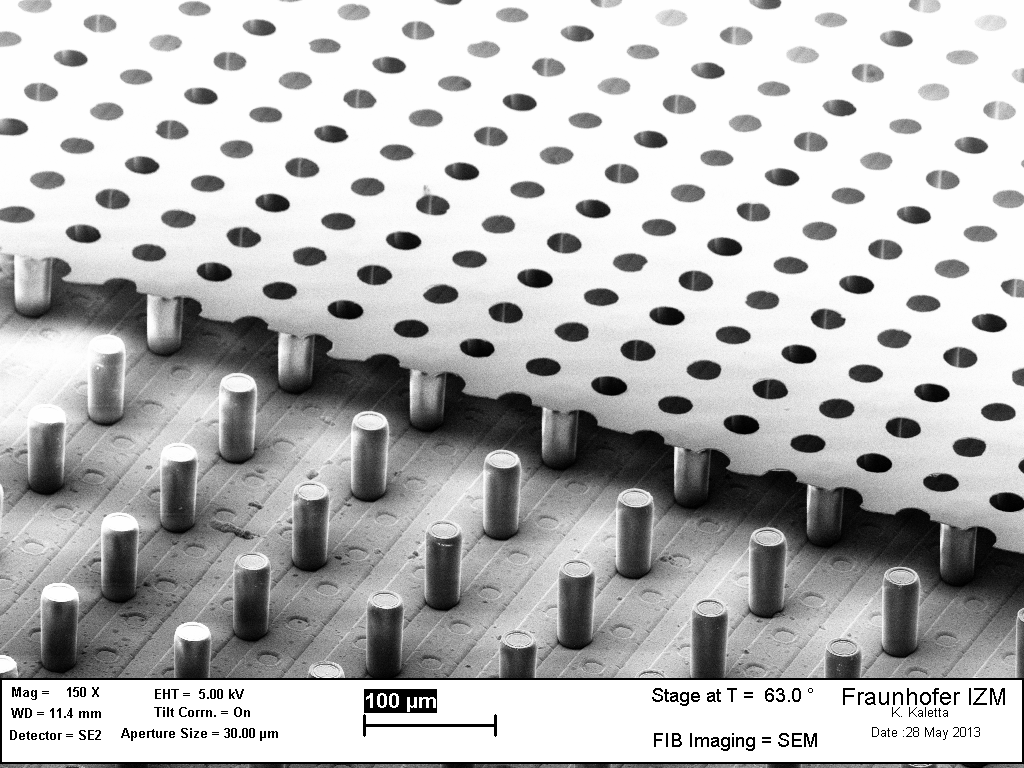
\includegraphics[width=0.45\textwidth]{Tracker/TPC_Bonn/plots/TPC_pixels_GridPix.png}
  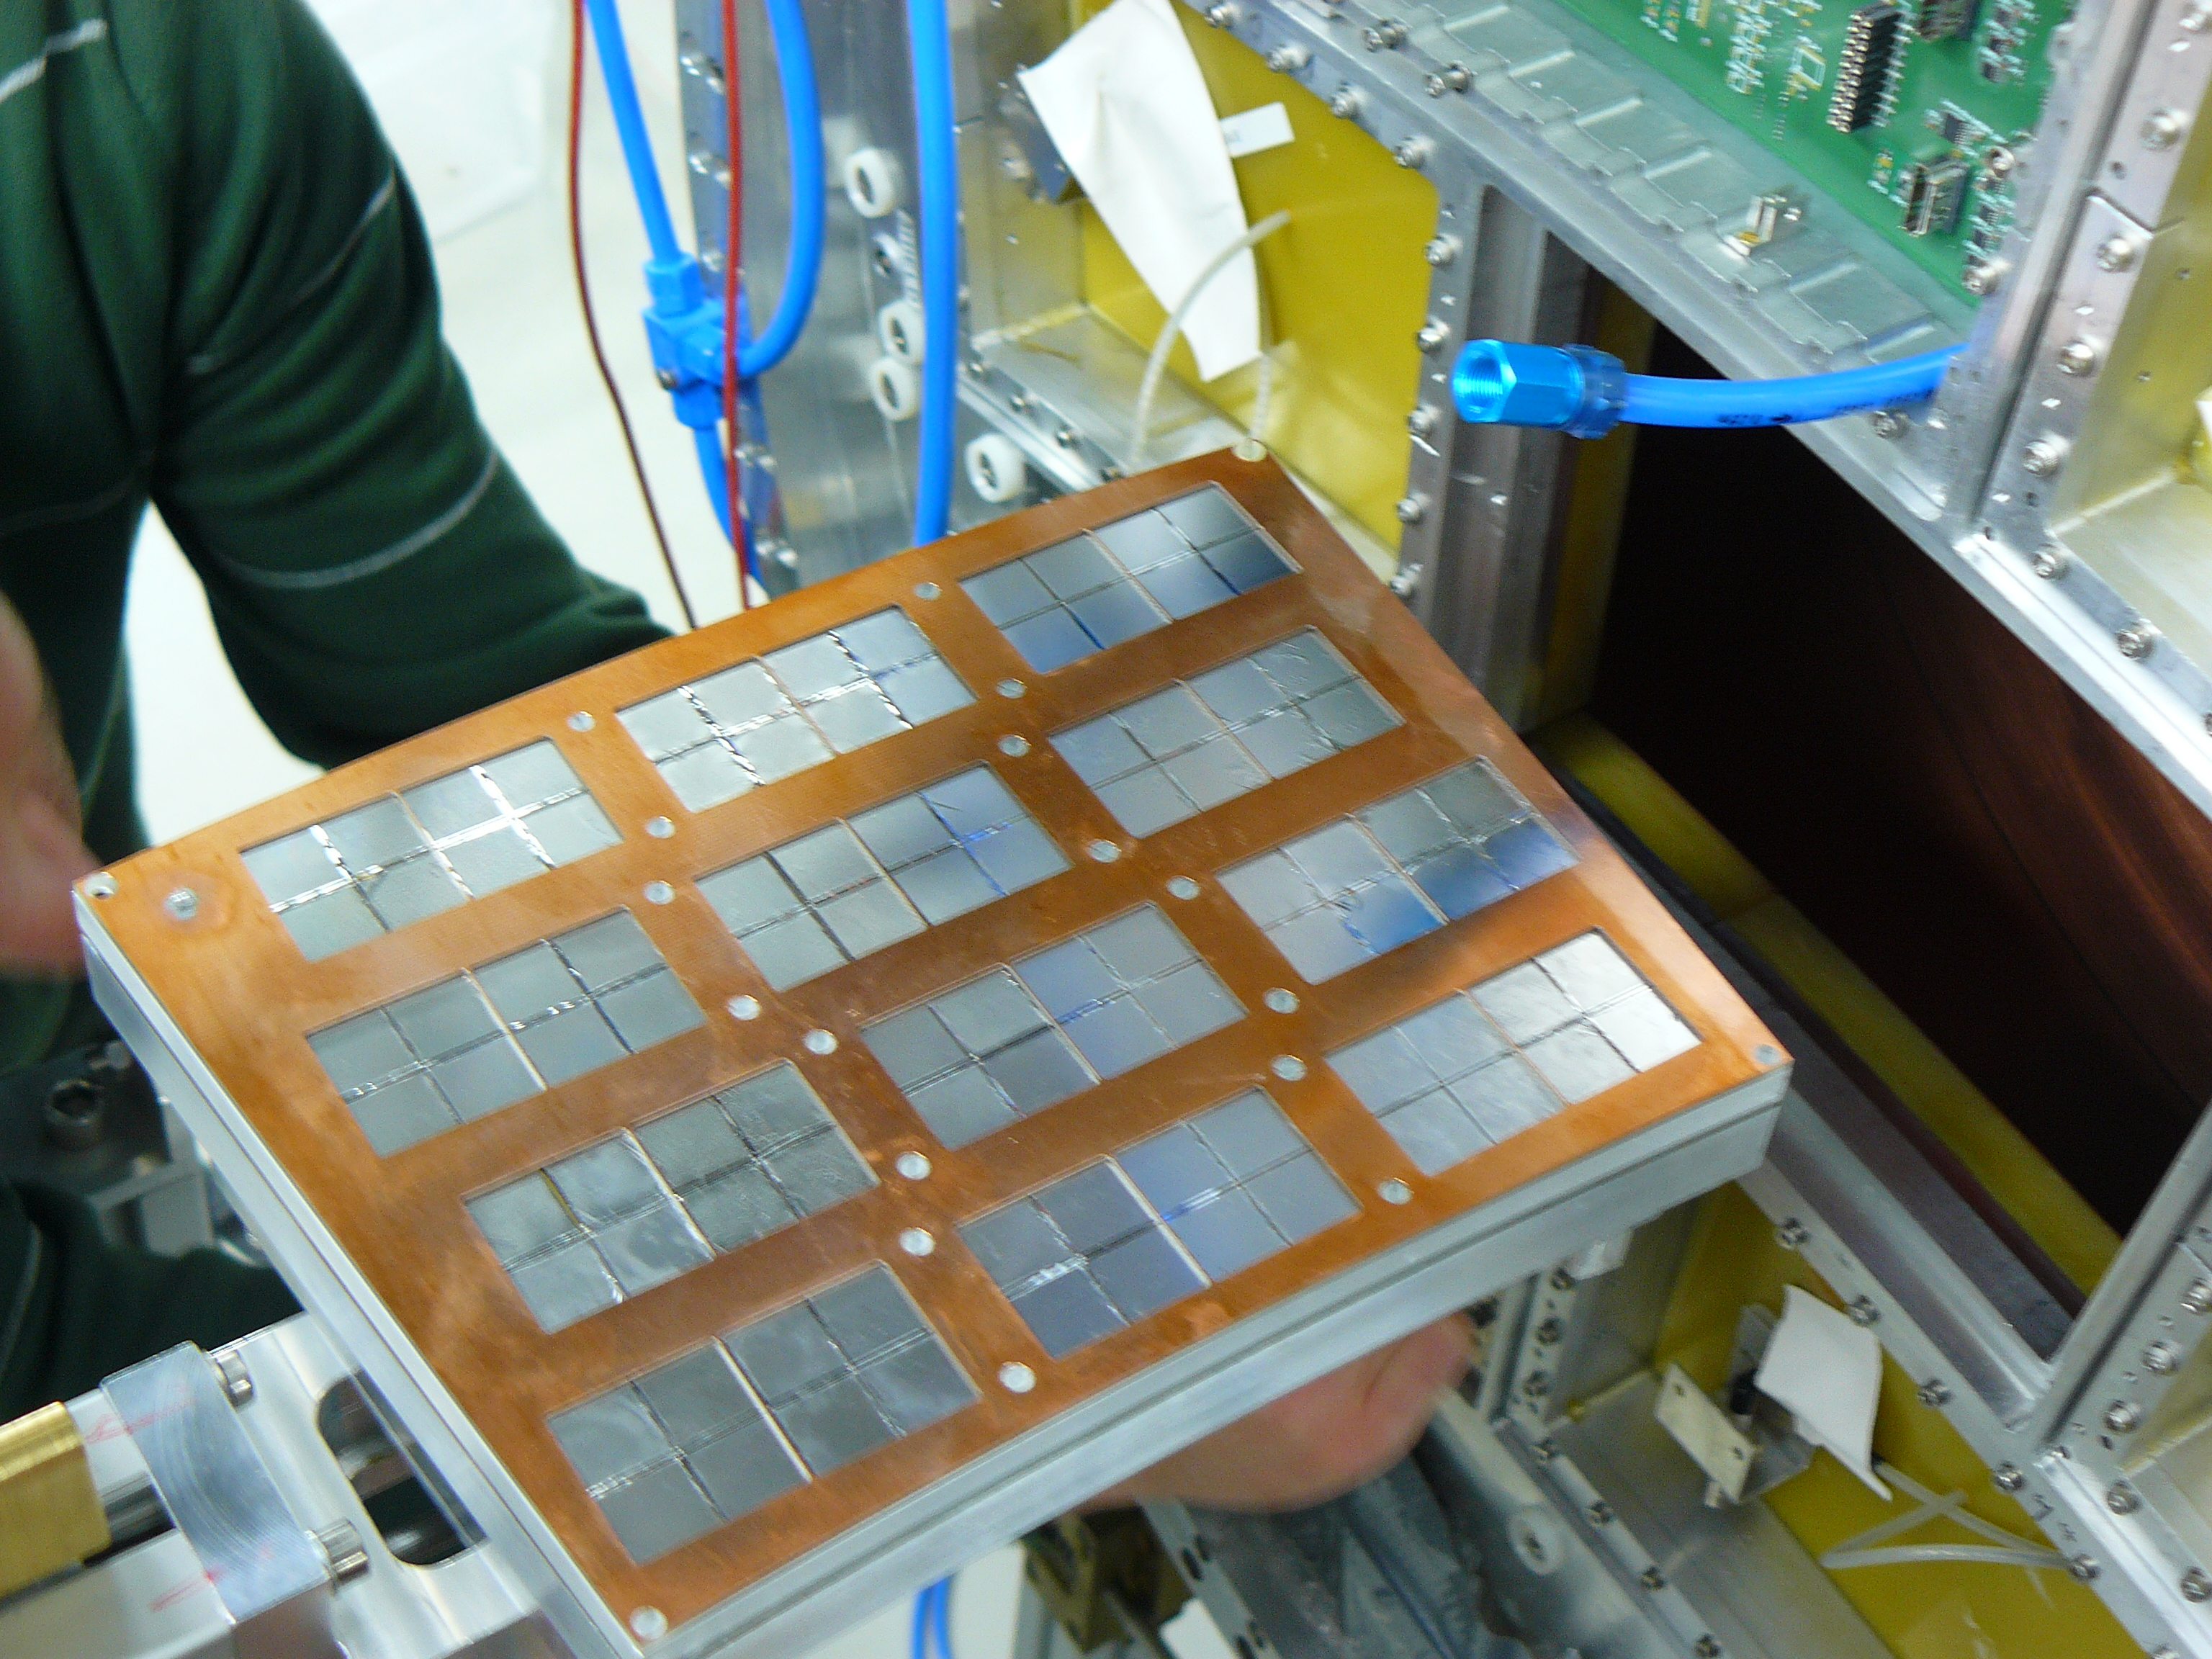
\includegraphics[width=0.45\textwidth]{Tracker/TPC_Bonn/plots/TPC_pixel_complete_module.png}
  \caption{Left: SEM picture of an InGrid detector with a partially removed
    grid, right: Fully equipped LP module with 96 GridPix detectors is being
    mounted in the LP.}
  \label{fig_TPC_pixels_1}
\end{figure}

This setup served as a demonstrator that larger areas ($\sim$\SI{400}{\centi\meter\squared}) could be produced and operated. It was tested in the Large Prototype in March/April of 2015 and operated for more than one week permanently in the
test beam. A total of about 200 runs with more than 1.5 million events were recorded \cite{7889045}.

\begin{figure}[!t]
  \centering
  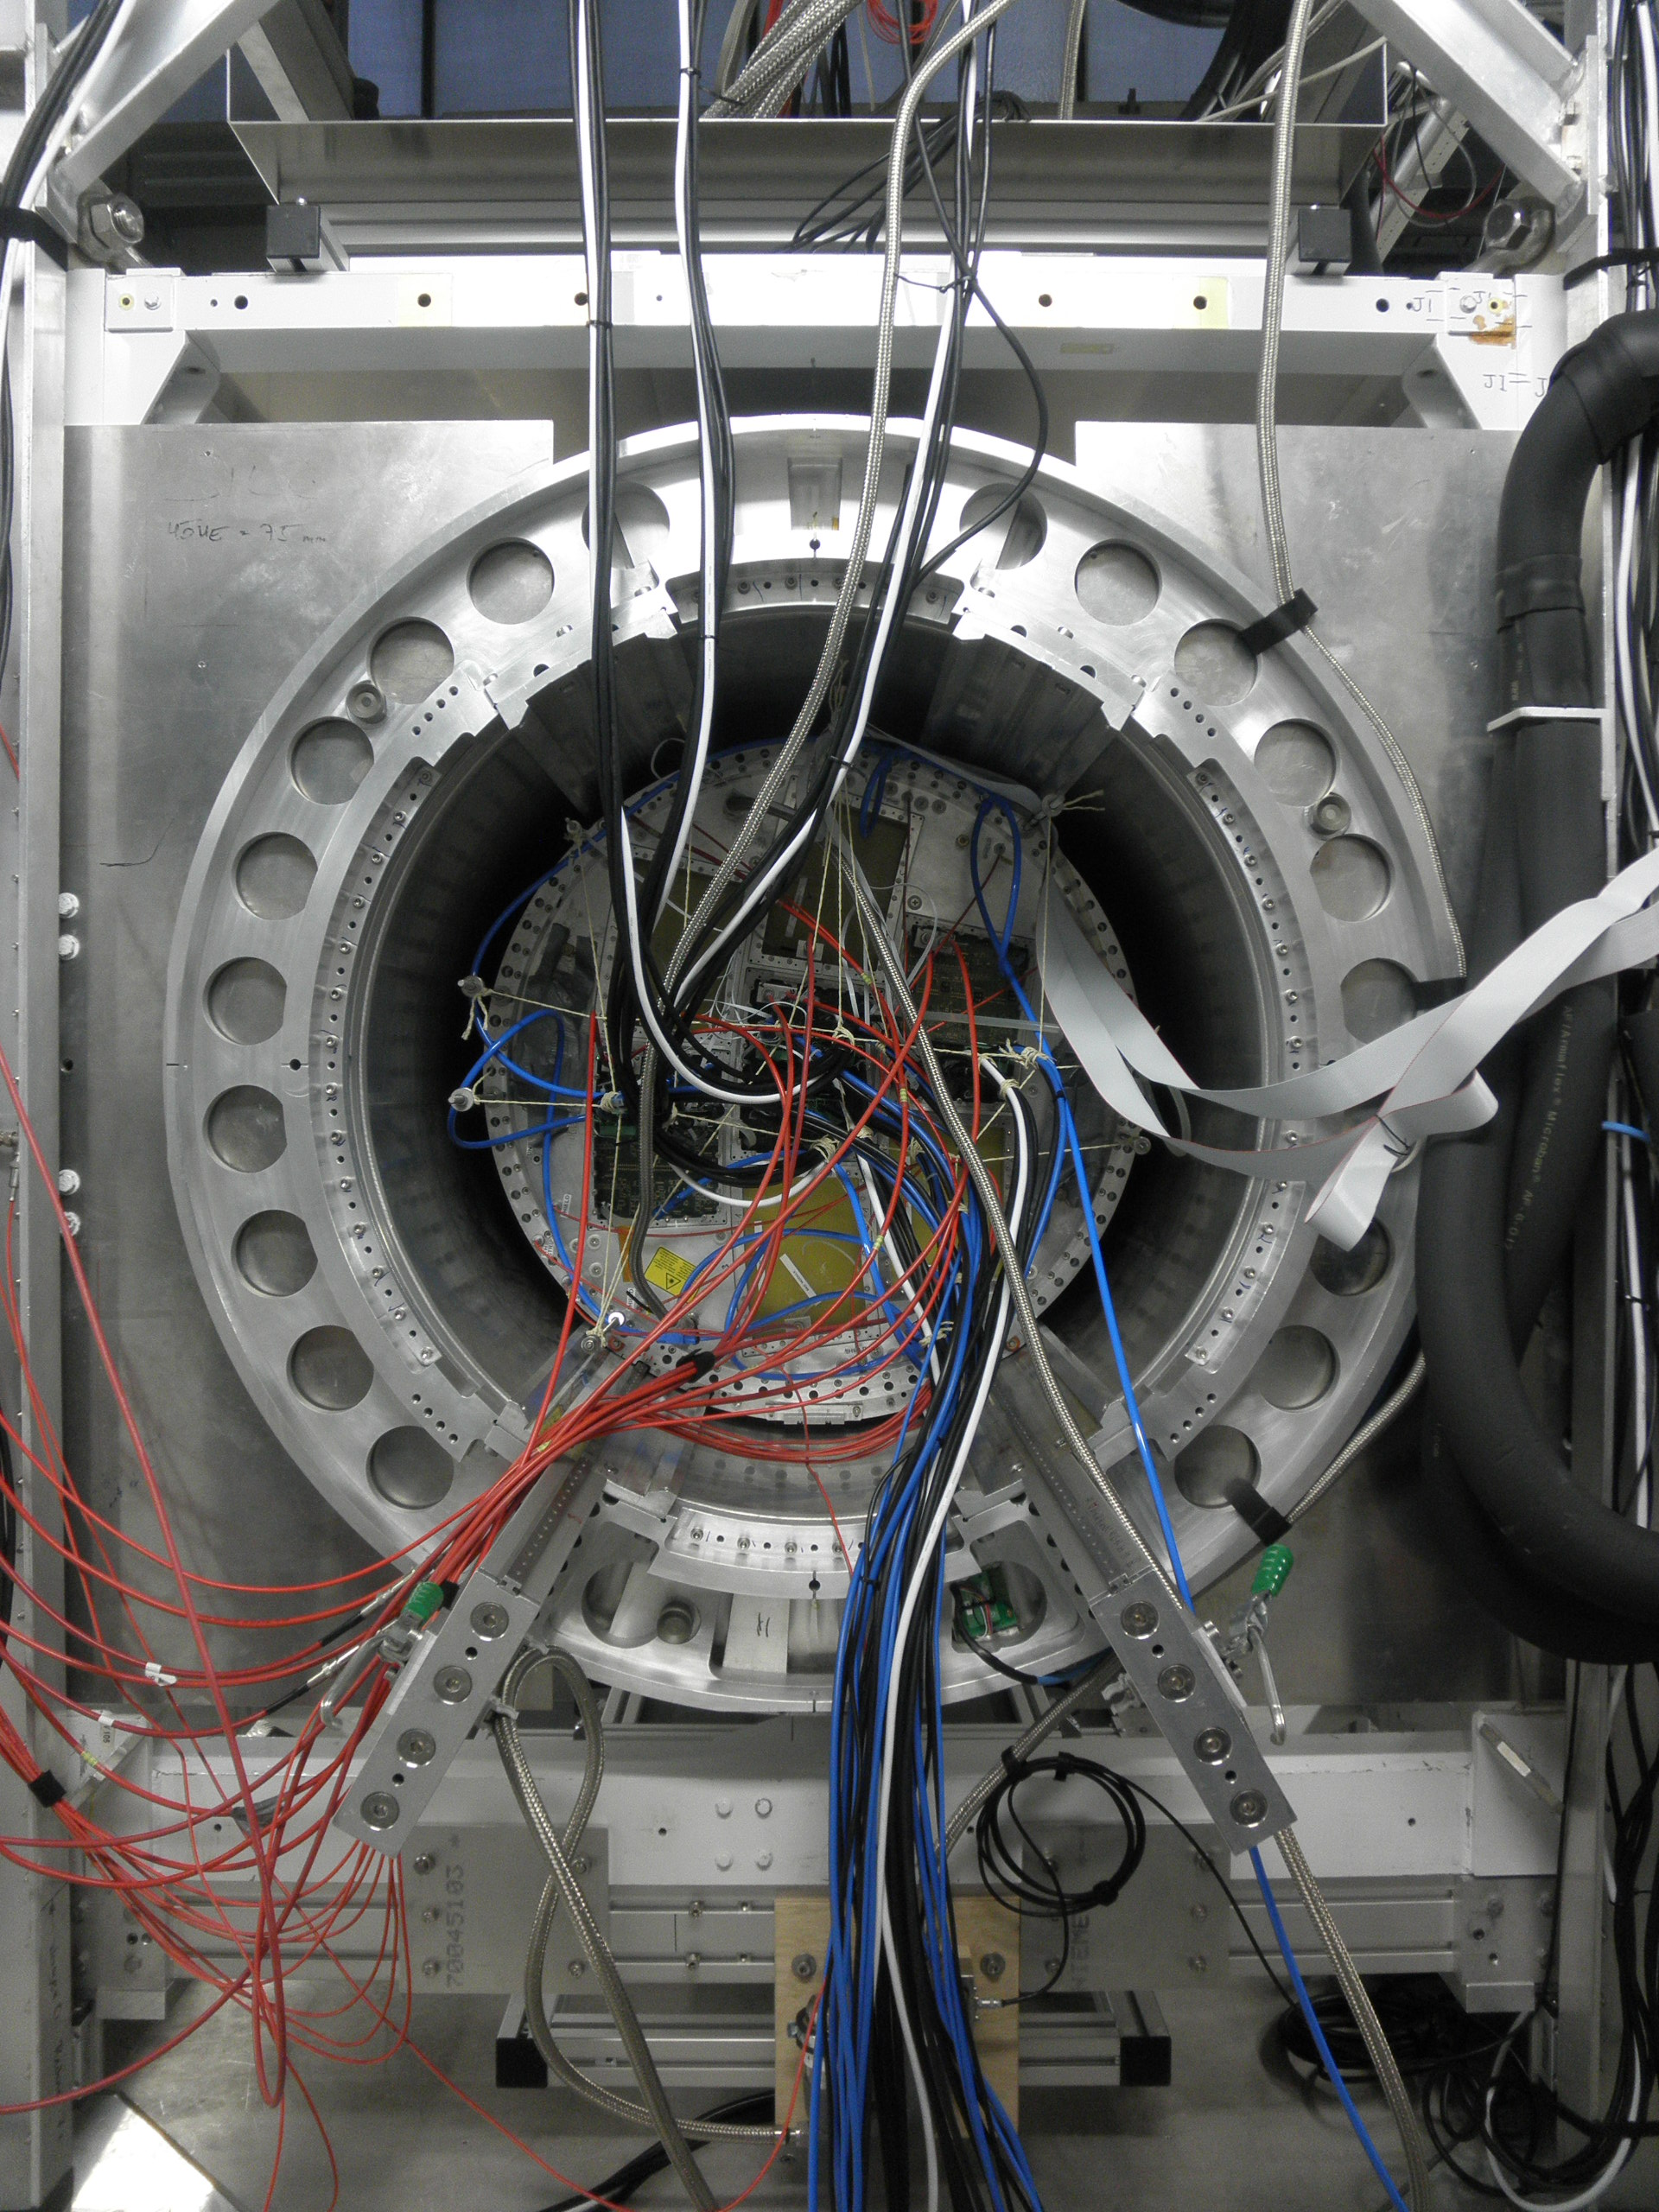
\includegraphics[width=0.28\textwidth]{Tracker/TPC_Bonn/plots/TPC_pixels_LP_GridPixes.png}
  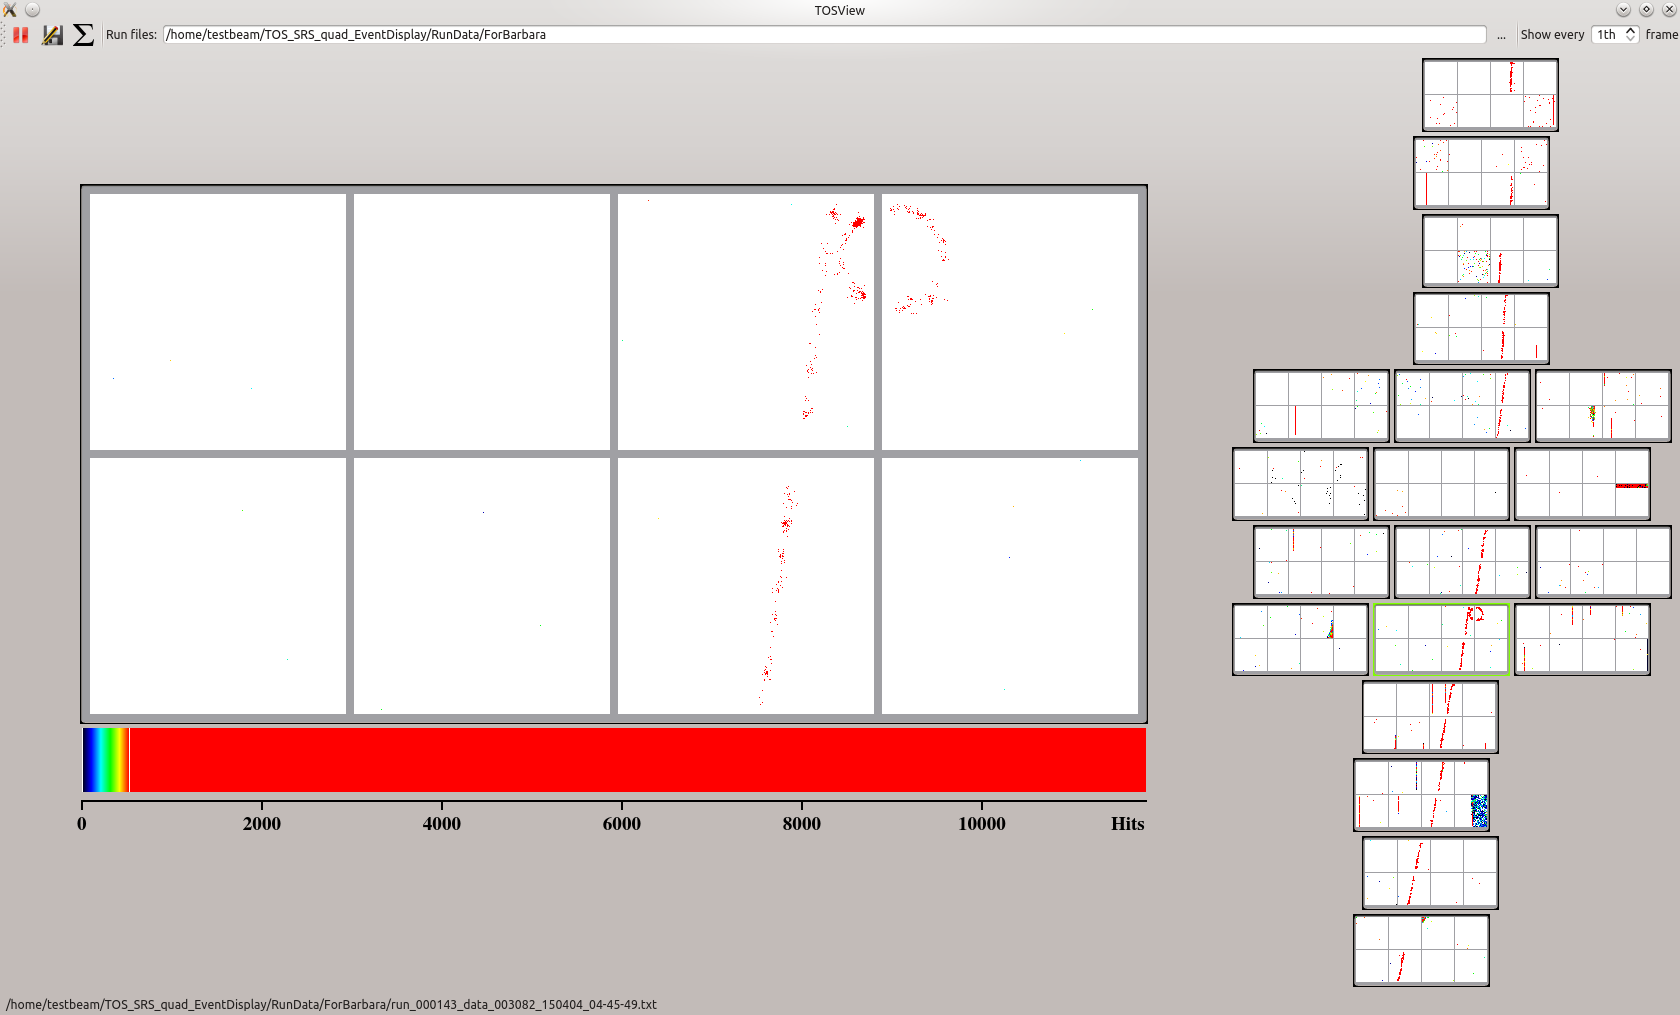
\includegraphics[width=0.62\textwidth]{Tracker/TPC_Bonn/plots/TPC_pixels_event.png}
  \caption{Left: Three modules with 160 GridPix detector mounted on the Large
    Prototype, right: Online event display of a 2 track event recorded with
    160 GridPixes.}
  \label{fig_TPC_pixels_2}
\end{figure}

Nikhef and Bonn have also taken part in designing a successor ASIC of
the currently used Timepix. The new Timepix-3 features several improvements,
which promise a much better performance. In particular it is multi-hit capable,
can record both time and charge of each signal, has a much faster
digitization frequency (\SI{640}{\mega\hertz}) and can be read out  quasi continuously.
Also, the grid design was revised increasing the active area to 97.7 percent of the pixel area. First Timepix-3-based GridPix detectors have been built and tested. A testbeam campaign was conducted in July 2017 at the ELSA accelerator in Bonn and a single GridPix detector was exposed to an 2.5 GeV electron beam \cite{Ligtenberg:2018sjs}. The performance clearly surpassed the one of Timepix-based GridPixes. In particular the longitudinal spatial resolution could be improved by over one order of magnitude. 

\subsection{Engineering Challenges}
The production of modules with large area coverage requires to solve four
major technical challenges: 
\begin{enumerate}
  \item The production of a large number of GridPixes with sufficiently good
quality. This has been addressed by the new production method, which is based
on complete wafers. The process was developed in collaboration with the
Fraunhofer Institute IZM at Berlin and yields up to 428 GridPixes per batch (4 wafers). 
\item In particular commercial readout systems are not easily scalable to a large number of chips. This is why Bonn has developed a cheap and easily expandable system based on the Scalable Readout System (SRS) of the RD51 collaboration.
Nikhef developed (partially funded by the AIDA FP7 project) the SPIDR fast readout system for Timepix-3 ASICs \cite{1748-0221-10-12-C12028}.
\item Current water cooling has to be replaced by 2-phase \ce{CO2} cooling.
\item In order to overcome systematic limitations of track reconstruction, field
  distortions caused by tilted chips and only partially covered ground
  potentials need to be mitigated.
\end{enumerate}

\subsection{Future Plans}
Currently the main focus is on the analysis of the test beam data. The
challenge of finding and fitting tracks with several thousand hits is quite
different from the standard pad-based TPC analysis. For this a group of people
from Nikhef, DESY, Siegen and Bonn are testing new ideas. On a longer term all
participating institutes are working on software to simulate, reconstruct and
analyze data of the ILD-TPC (i.e. about 10,000 hits per track) so that the
difference in performance between a pad and a pixel-based TPC can be studied. 
On the hardware side a new compact device containing four Timepix-3-based
GridPixes is being developed at Nikhef. This device called Quad minimizes the
dead area and new mounting procedures improve the alignment of the individual GridPixes,
so that a much reduced field inhomogeneity is expected. The construction of a
few fully equipped, engineering modules made of the aforementioned Timepix-3
GridPix Quads is planned.

\subsection{Applications Outside of Linear Colliders}
A seven GridPix detector is taking data for more than 1 year in the CAST
experiment for axion search and is also considered for the successor experiment IAXO.
In collaboration with KVI-CART in Groningen (NL) a system for proton radiography
is being developed using small (gaseous) TPCs based on GridPix detectors, for
accurate 3D proton tracking.

Also a new kind of neutron detector based on the TPC principle is being developed at Bonn. Here, a 8 GridPix readout at one of the endcaps is needed to reach the best possible spatial resolution.

Further applications in e.g. X-polarimetry and direction dark matter detection are envisaged.
